\def \Subject {سوال ۱: مدل‌های انتشار (DDPM/DDIM) و DreamBooth}
\def \Session { یک}
% \setcounter{chapter}{\Session-1}
\renewcommand{\chaptername}{سوال}
\chapter{\Subject}

در این بخش نتایج تجربی پیاده‌سازی
\grayBox{DDPM}
و
\grayBox{DDIM}
روی داده‌ی
\lr{CIFAR-10}
و هم‌چنین بخش دوم سوال یعنی
\grayBox{Stable Diffusion / DreamBooth}
گزارش می‌شود.

% ==========================
% بخش ۱: نتایج DDPM / DDIM
% ==========================
\section{نتایج مدل‌های انتشار روی CIFAR-10}

\subsection{نمونه‌های داده‌ی آموزشی و فرآیند افزودن نویز}

\begin{figure}[H]
    \centering
    \includegraphics[width=0.9\linewidth]{../En_report/figures/cifar_train_samples.png}
    \caption{نمونه‌ای از تصاویر آموزشی مجموعه‌داده \lr{CIFAR-10} که برای آموزش مدل انتشار استفاده شده‌اند.}
    \label{fig:cifar-train-samples}
\end{figure}

\noindent\textbf{توضیح شکل~\ref{fig:cifar-train-samples}:}
در این شکل چند نمونه تصادفی از تصاویر آموزش نشان داده شده است تا تنوع کلاس‌ها
(حیوانات، وسایل نقلیه و غیره)
و اندازه‌ی کوچک تصاویر \lr{(32×32)} مشخص شود.

\begin{figure}[H]
    \centering
    \includegraphics[width=0.9\linewidth]{../En_report/figures/forward_diffusion_noise.png}
    \caption{نمایش فرآیند پیش‌رونده‌ی افزودن نویز در مدل انتشار؛ با افزایش \lr{$t$}، تصویر به‌تدریج به نویز گاوسی خالص تبدیل می‌شود.}
    \label{fig:forward-diffusion}
\end{figure}

\noindent\textbf{توضیح شکل~\ref{fig:forward-diffusion}:}
این شکل نشان می‌دهد که چگونه در مراحل مختلف زمان \lr{$t$}، تصویر اصلی با نویز ترکیب شده و در مرحله‌ی نهایی تقریباً غیرقابل تشخیص می‌شود.

\subsection{منحنی خطای آموزش DDPM}

\begin{figure}[H]
    \centering
    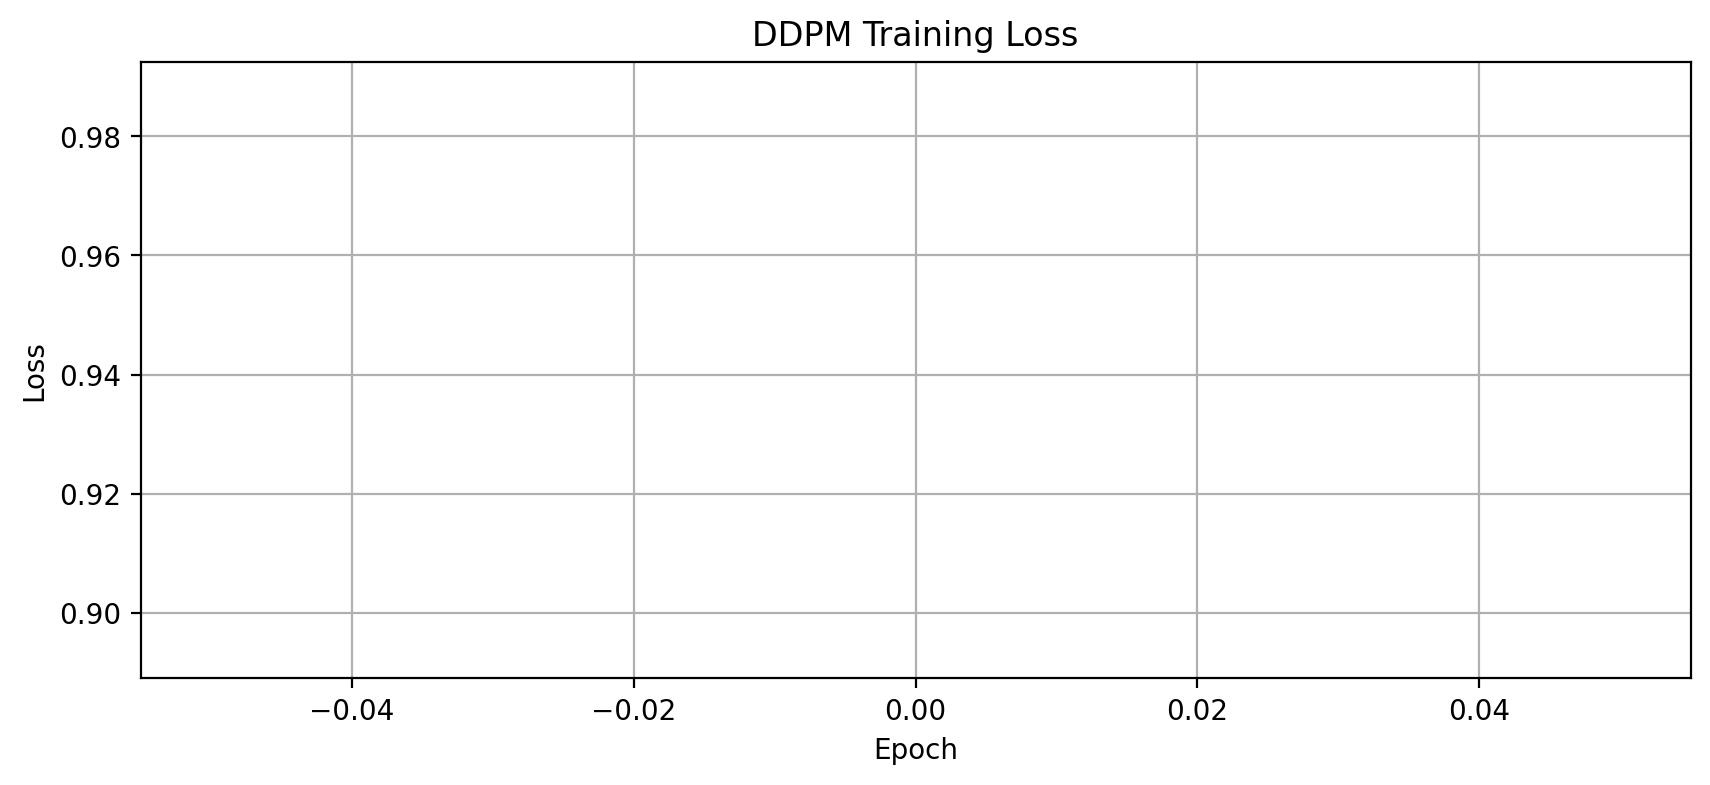
\includegraphics[width=0.8\linewidth]{../En_report/figures/ddpm_training_loss.png}
    \caption{منحنی خطای آموزش \lr{DDPM} (خطای \lr{MSE} پیش‌بینی نویز بر حسب دوره‌ی آموزش).}
    \label{fig:ddpm-train-loss}
\end{figure}

\noindent\textbf{توضیح شکل~\ref{fig:ddpm-train-loss}:}
همان‌طور که دیده می‌شود، خطای آموزش به‌صورت یکنواخت کاهش می‌یابد که نشان‌دهنده‌ی یادگیری پایدار مدل در پیش‌بینی نویز در گام‌های زمانی مختلف است.

\subsection{نمونه‌های تولیدشده توسط DDPM و DDIM}

\begin{figure}[H]
    \centering
    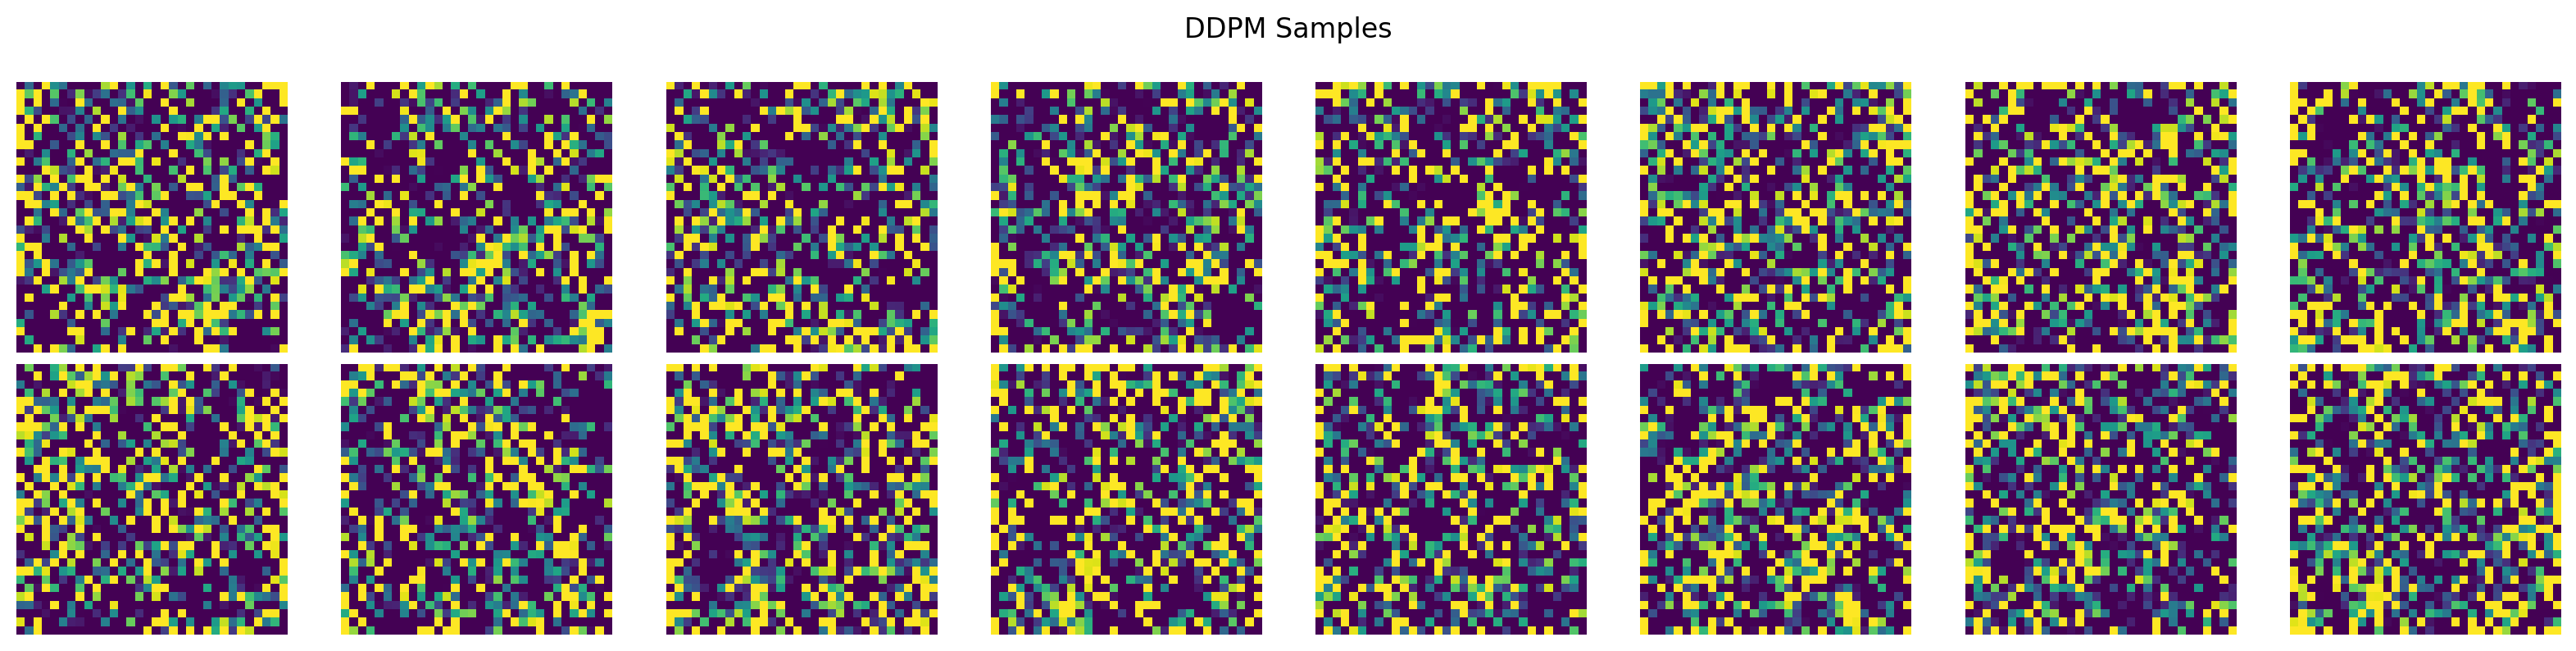
\includegraphics[width=0.9\linewidth]{../En_report/figures/ddpm_samples_grid.png}
    \caption{نمونه‌های تولیدشده توسط \lr{DDPM} با استفاده از تمام \lr{1000} گام معکوس.}
    \label{fig:ddpm-samples}
\end{figure}

\noindent\textbf{توضیح شکل~\ref{fig:ddpm-samples}:}
کیفیت تصاویر تولیدی مناسب بوده و ساختار اشیاء (مانند حیوانات و خودروها) قابل تشخیص است. به دلیل ماهیت تصادفی نمونه‌گیری، بین اجراهای مختلف تنوع نسبتاً خوبی مشاهده می‌شود.

\begin{figure}[H]
    \centering
    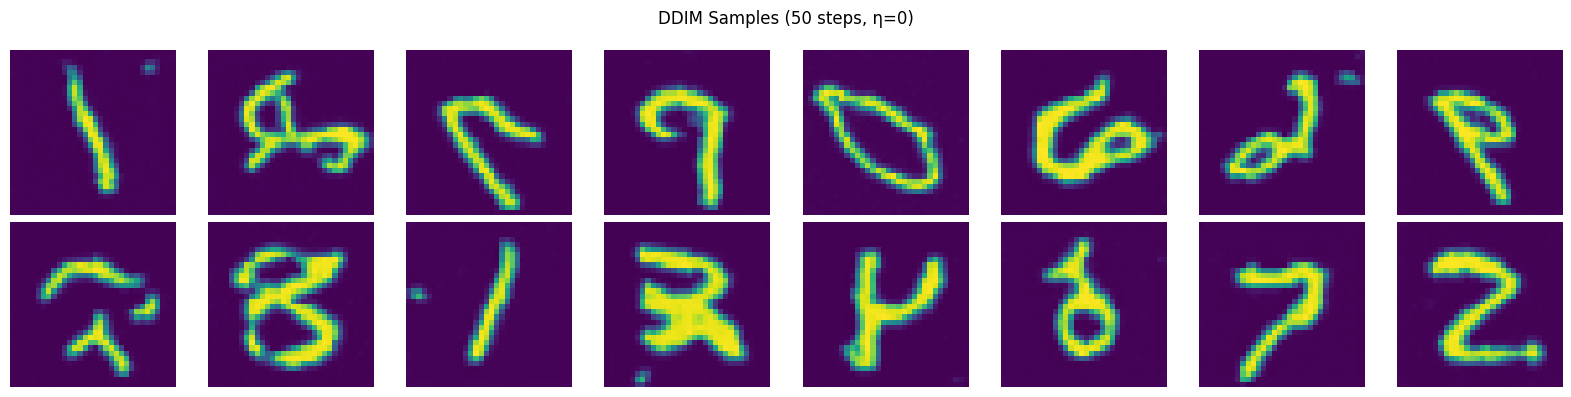
\includegraphics[width=0.9\linewidth]{../En_report/figures/ddim_samples_grid.png}
    \caption{نمونه‌های تولیدشده توسط \lr{DDIM} با \lr{50} گام و \lr{$\eta=0$} (نمونه‌گیری تعیین‌گر).}
    \label{fig:ddim-samples}
\end{figure}

\noindent\textbf{توضیح شکل~\ref{fig:ddim-samples}:}
در مقایسه با \lr{DDPM}، کیفیت تصاویر همچنان قابل قبول است در حالی که تعداد گام‌ها از \lr{1000} به \lr{50} کاهش یافته است؛ بنابراین سرعت نمونه‌گیری به‌طور محسوسی افزایش می‌یابد. تنظیم پارامتر \lr{$\eta$} امکان کنترل توازن بین تنوع و وفاداری را فراهم می‌کند.

% ==========================
% بخش ۲: نتایج DreamBooth
% ==========================
\section{نتایج Stable Diffusion و DreamBooth}

\subsection{تصاویر آموزشی و تعریف شناسه‌ی ویژه}

در این بخش، از چند تصویر چهره/سوژه‌ی شخصی استفاده شده و یک شناسه‌ی متنی خاص (برای مثال \grayBox{sks})
به آن اختصاص داده شده است تا مدل بتواند هویت سوژه را با این شناسه پیوند دهد.

\begin{figure}[H]
    \centering
    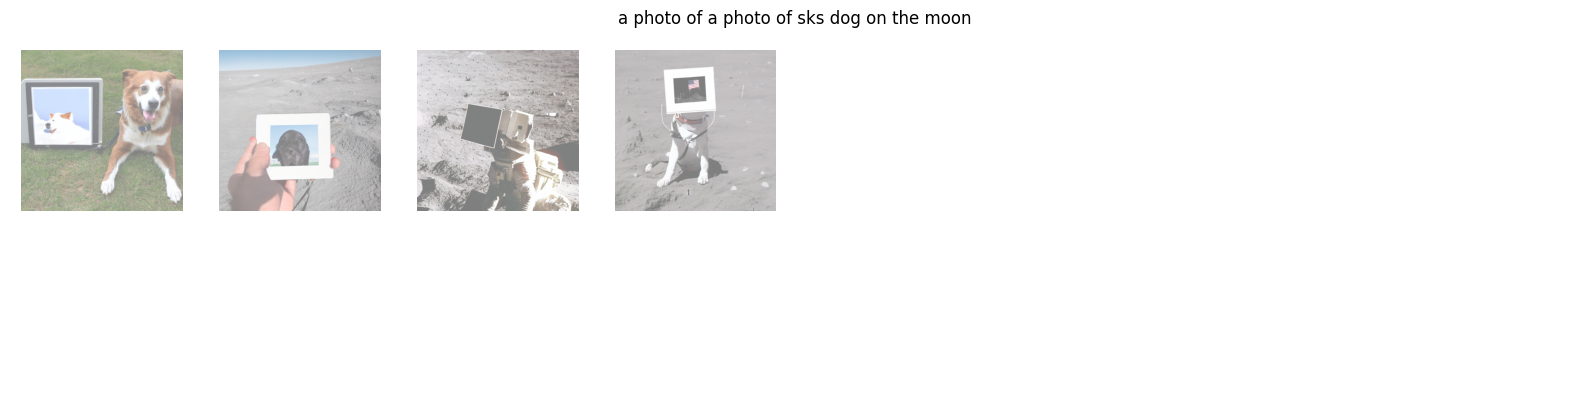
\includegraphics[width=0.45\linewidth]{../En_report/figures/dreambooth_instance_sample.png}
    \caption{نمونه‌ای از تصویر آموزشی که برای یادگیری سوژه با شناسه‌ی \grayBox{sks} استفاده شده است.}
    \label{fig:dreambooth-train}
\end{figure}

\noindent\textbf{توضیح شکل~\ref{fig:dreambooth-train}:}
این تصویر نمایان‌گر یکی از نمونه‌های آموزشی DreamBooth است؛ مشابه این تصویر چند نمای دیگر (زاویه‌ها و نورپردازی‌های متفاوت) نیز به مدل داده شده است.

\subsection{نمونه‌های تولیدی DreamBooth بعد از آموزش}

\begin{figure}[H]
    \centering
    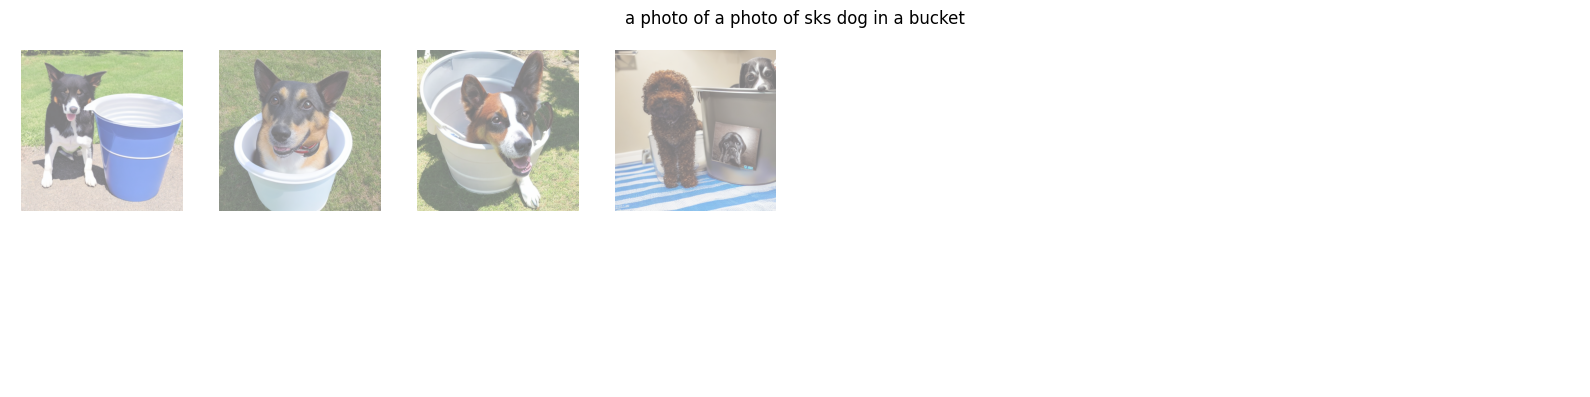
\includegraphics[width=0.9\linewidth]{../En_report/figures/dreambooth_generated_grid.png}
    \caption{شبکه‌ای از تصاویر تولیدی DreamBooth برای چند پرامپت شامل شناسه‌ی \grayBox{sks} (برای مثال «\lr{a photo of sks person in a fantasy landscape}»).}
    \label{fig:dreambooth-gen}
\end{figure}

\noindent\textbf{توضیح شکل~\ref{fig:dreambooth-gen}:}
مدل پس از پیش‌آموزش و ریزتنظیم با LoRA، قادر است سوژه‌ی مشخص را در سبک‌ها و صحنه‌های مختلف (واقعی و هنری) بازتولید کند؛ در عین حال ویژگی‌های چهره و هویت کلی سوژه تا حد خوبی حفظ می‌شود.

\vspace{0.5cm}
در ادامه، در سوال دوم (فایل \lr{session2.tex}) نتایج مدل \grayBox{Flow Matching} برای تولید سری‌های زمانی مالی گزارش می‌شود.
